\cleardoublepage
\chapter{Background}
\label{ch:chapter1}

\section{Robot Operating System}
\label{sec:chapter1:ros}
The \ac{ROS} \cite{ros-website} is an open source middleware that provides inter-process communication through a message passing mechanism. It is also a collection of libraries, tools and conventions with the aim of simplify the development of software for robots. In this sense, one of the main components of the framework are the nodes, which encapsulate processes and/or algorithms.

\subsection{Nodes}
\label{subsec:chapter1:ros:nodes}
Nodes are processes that perform a specific computation. In the system the nodes communicate between them using a publisher/subscriber infrastructure based on topics. A node subscribes to a particular topic, and it will receive messages from a publisher node. This way, a publisher node is hid to the subscriber, reducing the coupling between them. The advantage of this mechanism is that nodes can be developed separately once the message structure is defined, forcing developers to implement clear interfaces for communication by using a message \ac{IDL}. Moreover, this enables a modular and distributed development of the robotic system, while providing some fault tolerance and reduced code complexity.

\subsection{Topics}
\label{subsec:chapter1:ros:topics}
As mentioned before, communication between nodes is done via a publisher-subscriber architecture based on topics, which are named buses over which messages are exchanged. There can be several publishers (as well as subscribers) for a topic. A node that generates data publishes all its information in a specific topic bus, consequently this information is consumed by those nodes subscribed to that topic. The transport protocol used for exchanging messages is defined at runtime and can be of two types: TCPROS or UDPROS. The description of these protocols is beyond the scope of this document and the reader is invited to read the \ac{ROS} documentation for detailed information.

\begin{figure}
    \centering
    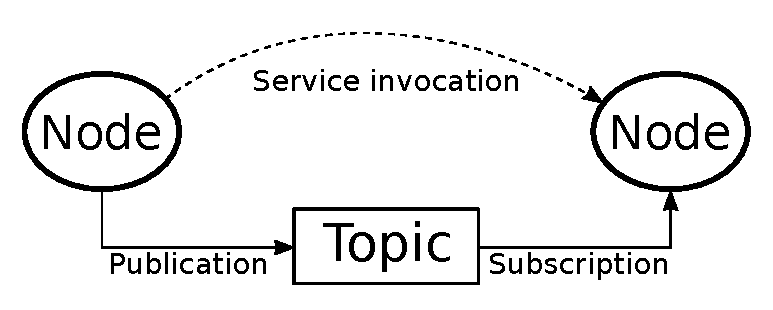
\includegraphics[width=0.7\linewidth]{Images/fig13-ros-basic-concept.eps}
    \caption[ROS basic concept]{\ac{ROS} basic concepts. Two nodes communicate between them using the messages published in a topic. One node is responsible of publishing the topic, while the other subscribes and receives the messages of that particular topic. Furthermore, the node in the left calls a service provided by the node in the right, so that node will perform some computation and will return the result. \cite{ros-website}}
    \label{fig:chapter1:ros:basic_concepts}
\end{figure}

\subsection{Services}
\label{subsec:chapter1:ros:services}
As well as topics, services are a way to communicate nodes. The difference is that topics are an asynchronous way of communication, while services are synchronous. The key difference lies on the ability of nodes to decide when to trigger a service. Hence, services are used in between nodes to retrieve specific information or to request another node to carry out a computation beyond caller's node scope.


\subsection{Tools}
\label{subsec:chapter1:ros:tools}
Regarding the tools provided by \ac{ROS}, one that is crucial for debugging and/or experimentation is the bag recording and playback. Since the exchange of messages between nodes is anonymous (meaning that nodes communicate between each others without knowing which node sent or received a message) it is possible to record the messages during a period of time, without taking into consideration which node sent a message and which node received it. This recorder bag is useful for debugging since it can be played back, hence reproducing a previous experiment. Also, it can be used for the development of new nodes that depend on the messages contained in the bag.\\

Another useful tool provided is \ac{RViz}, a 3D visualization tool. With this tool it is possible to see the robot, orientation, reference frames, covariance matrices, etc. In addition, it is possible to draw lines, arrows, text and others, onto the environment in order to see useful information that cannot be extracted from messages.

\subsection{MAVLink and MAVROS}
\label{sssec:chapter2:drone:mavlink}
%\nocite{mavlink}
MAVLink \cite{mavlink} is a binary telemetry protocol designed for resource-constrained systems and bandwidth-constraint links, more specifically for drones of all kinds. As with \ac{ROS}, it adopts a publisher-subscriber architecture, where data streams are published as topics. MAVLink key features, as published in its website are:
\begin{itemize}
    \item Since its messages do not require any special framing, it is well suited for applications with very limited bandwidth.
    \item It provides methods for detecting package drops, corruption and for package authentication.
    \item Allows up to 255 concurrent systems on the network.
    \item Enables both offboard and onboard communications.
\end{itemize}
%\nocite{mavros}
MAVROS \cite{mavros} is the extension of MAVLink in \ac{ROS}, with the addition of being a proxy for Ground Control Station tool. Its main features, as published in its website are:
\begin{itemize}
    \item Communication with autopilot via serial port, UDP or TCP .
    \item Internal proxy for Ground Control Station (serial, UDP, TCP).
    \item Plugin system for ROS-MAVLink translation.
    \item Parameter manipulation tool.
    \item Waypoint manipulation tool.
    \item PX4Flow support (by mavros\_extras).
    \item OFFBOARD mode support.
\end{itemize}

One characteristic that is worth mentioning, is that MAVROS translates the \ac{NED} reference frames into \ac{ENU} reference frames, and vice-versa, so as to be compliant with \ac{ROS} standard reference frames.

\subsection{RTAB-Map}
\label{subsec:chapter1:ros:octomap}
\ac{RTAB-Map} is a RGB-D, stereo and LiDAR graph-based \ac{SLAM} approach based on an incremental appearance-based loop closure detector. It allows to build a 3 dimensional map of the environment using a stereo camera, a LiDAR sensor and/or the odometry estimation. The map is built using a 3D occupancy grid by means of Octomap library, which builds a tree-based representation of the mapped area. Octomap library \enquote{performs a probabilistic occupancy estimation to ensure updatability and to cope with sensor noise}\cite{octomap-paper}.\\

\begin{figure}
    \centering
    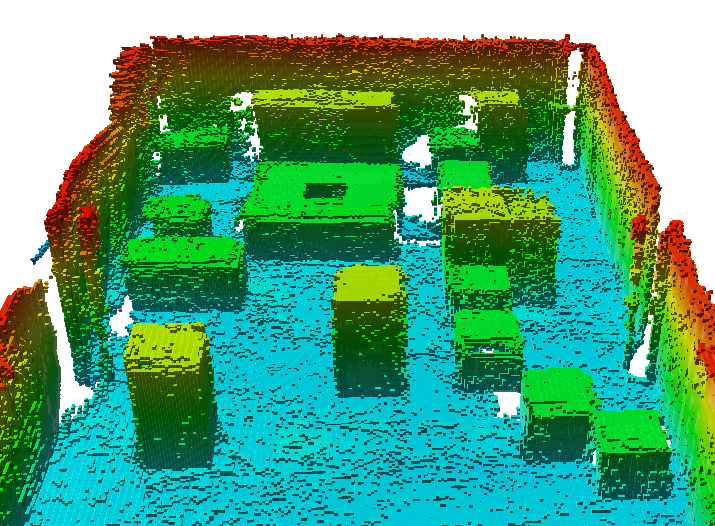
\includegraphics[width=\textwidth]{Images/fig14-octomap-colored2.png}
    \caption[Octomap example]{Octomap example. Octotree representation generated from data, showing occupied voxels only. \cite{octomap-paper}}
    \label{fig:chapter1:ros:octomap}
\end{figure}


The Octomap library generates an octotree, which is a hierarchical data structure used to generate spacial subdivision in 3 dimensions. Each node in an octotree represents a voxel, which is a cubic volume, which is at the same time, subdivided in eight smaller cubes until a given minimum voxel size called resolution. This way, the octotree data structure is used to build an occupancy grid of a volume. An example of a octotree can be seen in Figure~\ref{fig:chapter1:ros:octomap}, where the color of each occupied voxel represents its height: higher voxels are red-colored, while lower voxels are light-blue-colored.\\

\ac{RTAB-Map} library, uses the Octomap library to store the 3D occupancy grid of the environment. The \inlinesrc{rtabmap_ros} node is the extension of the \ac{RTAB-Map} library for \ac{ROS}. It uses the information of a stereo camera or a RGB-D camera and/or a LiDAR information to create a cloud point that is used to build the map. Furthermore, it uses the provided odometry to estimate and correct the robot's pose into the 3D map. An example of this procedure can be seen in Figure~\ref{fig:chapter1:ros:rtabmap}.

\begin{figure}
    \centering
    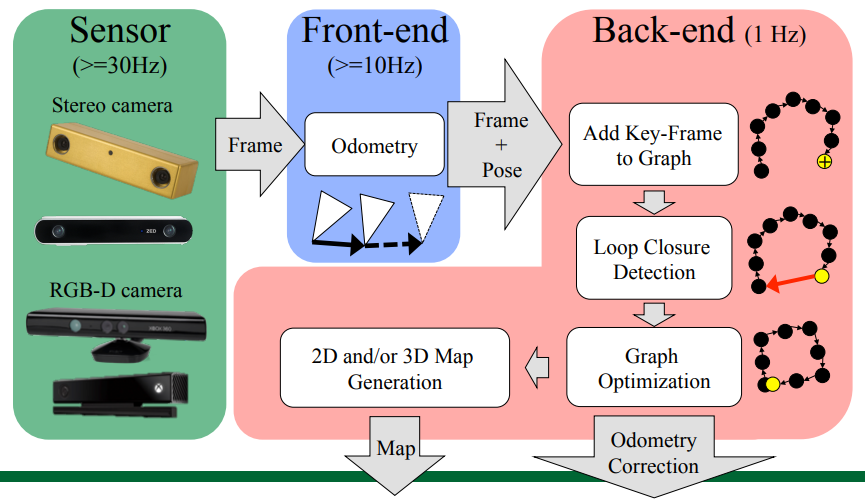
\includegraphics[width=\textwidth]{Images/fig14-rtabmap3.png}
    \caption[RTAB-Map example]{\ac{RTAB-Map} example. An stereo camera or a RGB-D camera is used among the odometry estimation. Both are used to generate a 3D occupancy grid using Octomap library, and to correct the odometry estimation. \cite{rtabmap-presentation}}
    \label{fig:chapter1:ros:rtabmap}
\end{figure}

\section{Transformations}
\label{sec:chapter1:transform}
A robot, in this case the drone, can be considered as a rigid body that moves and rotates around the environment. Hence, it is necessary to model the drone displacement in space, and this can be done by decomposing the movement as translations and rotations.

\subsection{Translation}
\label{subsec:chapter1:transform:translation}
Given a vector $\bm{b} = \begin{bmatrix}b_x & b_y & b_z\end{bmatrix}^T$ that represents the center of mass of a rigid body, a translation that displaces $\bm{b}$ parallel to itself of a given vector $\bm{t}$ can be defined as:
\begin{align*}
    \bm{b} + \bm{t} = \begin{bmatrix}
        b_x \\ b_y \\ b_z
    \end{bmatrix} + \begin{bmatrix}
    t_1 \\ t_2 \\ t_3
\end{bmatrix} = \begin{bmatrix}
        b_x + t_1\\ b_y + t_2 \\ b_z + t_3
\end{bmatrix}~~.
\end{align*}
Given a point $P$ represented in the reference frame $\mathcal{R}_m$ by $\bm{v_P^m}$ will be represented in the reference frame $\mathcal{R}_n$ by:
\begin{align*}
    \bm{v_P^n} = \bm{v_P^m} + \bm{t_m^n}~~,
\end{align*}
where $\bm{v_P^n}$ is the vector that represents the point $P$ in the reference frame $\mathcal{R}_n$, $\bm{v_P^m}$ is the vector that represents the point $P$ in the reference frame $\mathcal{R}_m$, and $\bm{t_m^n}$ is the vector that represents the translation from reference frame $\mathcal{R}_n$ to reference frame $\mathcal{R}_m$.

\subsection{Rotation}
\label{subsec:chapter1:transform:rotation}
In three dimensional space, any displacement of a rigid body is equivalent to a single rotation of a given angle about some axis that contains the point. It is possible to express the previous statement as $\bm{v} = \bm{u} * \theta$, being $\bm{u}$ a unit vector representing the axis and $\theta$ the angle.\\

Unlike with translations, two or more rotations cannot be simply the sum of the related vectors. A rotation can be described assuming a rigid body in a reference frame with its origin fixed, while the unit vectors are changed under the rotation. This way, a rotation is characterized by the mathematical relation of these two reference frames. Hence, in order to represent a rotation, two reference frames with a common origin are needed, as shown in Figure~\ref{fig:chapter1:transformation:rotation:3d-example}. At the beginning the two reference frames coincide, then one of them is rotated around the origin by an arbitrary angle. After this procedure, the two reference frames are not coincident anymore, however, both share the same origin.\\

\begin{figure}
    \centering
    \includegraphics[width=\textwidth]{Images/fig17-3D-rotation-example}
    \caption[Rotation around origin]{Rotation around origin. The reference frame at the left is rotated around Y axis and, as result, a new reference frame is obtained, both sharing the same origin.}
    \label{fig:chapter1:transformation:rotation:3d-example}
\end{figure}

The rotation by any angle around any axis can be represented in a matrix form, $\bm{R_n^m}$, where each column of the matrix represents the unit vector of $R_n$ in $R_m$, so it represents the rotated frame $R_n$ with respect the fixed frame $R_m$ with common origin. Furthermore, it is possible to show that matrix $\bm{R_n^m}$ is \emph{orthonormal}, which means that its inverse is equal to its transpose.\\

Given the matrix representation of a rotation, it is possible to provide a way to rotate a vector in the space. When the reference frames origins are the same, the rotation of a vector is possible by multiplying it by the rotation matrix around an axis: $\bm{v^m} = \bm{R_n^m} \bm{v^n}$. This kind of rotations are called \emph{elementary rotations}, and given that there are three axis in a 3D space, three different elementary rotations can be defined:
\begin{enumerate}
    \item{Rotation around axis $x$: \begin{align*}
            \bm{R_{x, \theta}} = \begin{bmatrix}
                1 & 0 & 0 \\ 0 & \cos{\left(\theta\right)} & -\sin{\left(\theta\right)} \\ 0 & \sin{\left(\theta\right)} & \cos{\left(\theta\right)}
            \end{bmatrix}~~.
    \end{align*}}
    \item{Rotation around axis $y$: \begin{align*}
        \bm{R_{y, \theta}} = \begin{bmatrix}
             \cos{\left(\theta\right)} & 0 &  \sin{\left(\theta\right)} \\ 0 & 1 & 0 \\  -\sin{\left(\theta\right)} & 0 & \cos{\left(\theta\right)}
        \end{bmatrix}~~.
    \end{align*}}
    \item{Rotation around axis $z$: \begin{align*}
        \bm{R_{z, \theta}} = \begin{bmatrix}
            \cos{\left(\theta\right)} & -\sin{\left(\theta\right)} & 0 \\ \sin{\left(\theta\right)} & \cos{\left(\theta\right)} & 0 \\ 0 & 0 & 1
        \end{bmatrix}~~.
    \end{align*}}
\end{enumerate}

As mentioned, unlike translations, rotations cannot be summed. Hence, if two consecutive rotations need to be performed around two axis, a multiplication is needed:
\begin{align}
    \bm{R_{z,x}} = \bm{R_{x, \alpha}} * \bm{R_{z, \beta}}~~,
\end{align}
where $\bm{R_{z,x}}$ is the rotation around axis $z$ by an angle $\beta$ followed by a rotation around the new axis $x$ by an angle $\alpha$, as shown in Figure~\ref{fig:chapter1:transform:rotation_z_x}.

\begin{figure}
    \centering
    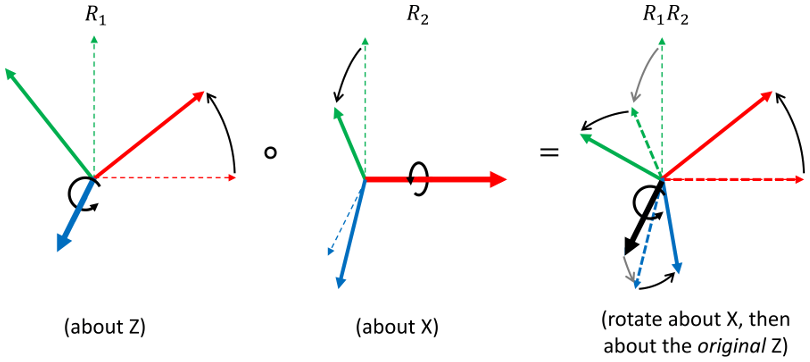
\includegraphics[width=\textwidth]{Images/fig16-rotations.png}
    \caption[Rotation around axis $z$ followed by rotation about axis $x$]{Rotation about axis $z$ followed by rotation about axis $x$. The second rotation is performed about the original axis $z$. This final rotation can be achieve by multiplying $R_1$ and $R_2$.\cite{hauser-robotics-systems}}
    \label{fig:chapter1:transform:rotation_z_x}
\end{figure}

\subsection{Homogeneous transform}
\label{subsec:chapter1:transform:rototranslation}
A rotation and a translation can be accomplished as follow: $\hat{\bm{v}} = \bm{R}\bm{v} + \bm{t}$. Nevertheless, this can be achieve by using \emph{homogeneous coordinates}, where the point $\bm{v}$, expressed in its homogeneous representation, is $\bm{v} = \begin{bmatrix}v_x & v_y & v_z & 1\end{bmatrix}^T$. This way, the rotation and translation of a point can be accomplished by multiplying the 3D point with the homogeneous transformation matrix:
\begin{align}
    \bm{T}_m^n &= \begin{bmatrix}
        \bm{R}_m^n & \bm{t} \\
        \bm{0} & 1
    \end{bmatrix}~~,
    \label{eq:chapter1:transform:homogeneous_transform}\\
    \hat{\bm{v}}^n &= \bm{T}_m^n\bm{v}^m~~.
\end{align}
The rotation component of $\bm{T}_m^n$ needs to be defined. Several definitions are possible, and in this work the \emph{RPY} order is used. RPY order of rotations establishes the order of the rotations applied to the three axis given three different angles. Therefore, $\bm{R}_m^n$ is a sequence of rotations around the X axis, Y axis and Z axis, given $\phi$, $\theta$ and $\psi$ angles, which is the same as $R_{z,\psi}R_{y,\theta}R_{x,\phi}$.\\

As can be noticed in equation~(\ref{eq:chapter1:transform:homogeneous_transform}), the homogeneous transformation is represented by a $4 \times 4$ matrix, and unlike the pure rotation matrix showed in Section~\ref{subsec:chapter1:transform:rotation}, the inverse of the homogeneous transformation is not equal to its transpose. The inverse of the homogeneous transformation is equivalent to:
\begin{align}
    \bm{T}^{-1} &= \begin{bmatrix}
        \bm{R}^T & -\bm{R}^T\bm{t} \\
        \bm{0} & 1
    \end{bmatrix}~~.
\end{align}

\begin{figure}
    \centering
    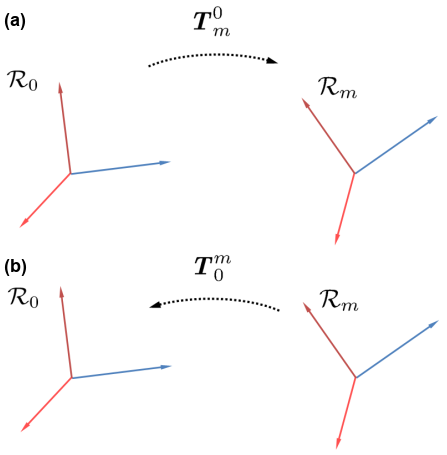
\includegraphics[width=0.5\textwidth]{Images/fig15-homogeneous-transform.png}
    \caption[Example of a Homogeneous transform]{Example of a Homogeneous transform. \textbf{(a)} Transformation $\bm{T}_m^0$ is applied to a point in reference frame $\mathcal{R}_0$ to express it in reference frame $\mathcal{R}_m$. \textbf{(b)} The inverse transformation is applied, so to express the point in reference frame $\mathcal{R}_m$ into reference frame $\mathcal{R}_0$.  \cite{bona-dynamic-modelling}}
    \label{fig:chapter1:transform:homogeneous}
\end{figure}

\section{Kalman Filter}
\label{sec:chapter1:kf}
%\nocite{intro-robotics}

Introduced by \cite{kalman}, the \ac{KF} provides a recursive method for estimating the state of a dynamic system with presence of noise. It is a technique for filtering and prediction in \emph{linear Gaussian systems} and applicable only to continuous states. One of its key features is that it simultaneously maintains estimates of the state vector and the estimate error covariance. It assures that the posteriors are Gaussian if the Markov assumption is hold, in addition to three conditions. The Markov assumption states that the past and future data are independent if one knows the current state; the other three conditions are the following:
\begin{enumerate}
    \item{The state transition probability $p\left( x_t | u_t, x_{t-1}\right)$ must be a linear function in its arguments. This is guaranteed by $ x_t = A_t x_{t-1} + B_t u_t + \epsilon_t $. Here, $x_t$ and $x_{t-1}$ are the state vectors of size $n$, and $u_t$ represents the control vector of size $m$ at time $t$; $A_t$ and $B_t$ are matrices of size $n \times n$ and $n\times m$ respectively. In this way, the state transition function becomes linear in its arguments, hence \ac{KF} assumes a linear system dynamics. $\epsilon_t$ represents the uncertainty introduced by the state transition, and it is a Gaussian random variable with zero mean and $R_t$ covariance.}
    \item{The measurement probability $p\left(z_t | x_t\right)$ must be linear in its arguments. This is guaranteed by $z_t = C_t x_t + \delta_t$, where $z_t$ represents the measurement vector of size $k$, $C_t$ is a matrix of size $k \times n$ and $\delta_t$ is a Gaussian noise with zero mean and $Q_t$ covariance.}
    \item{The initial belief should be normally distributed.}
\end{enumerate}
Given these three conditions, we are guaranteed that the posterior probability is Gaussian.\\
\begin{algorithm}[h]
    \caption{Kalman Filter algorithm}
    \label{alg:chapter1:kf}

    \BlankLine
    \KwIn{$\mu_{t-1}$, $\Sigma_{t-1}$, $u_t$, $z_t$}
    \BlankLine
    $\hat\mu_t = A_t \mu_{t-1} + B_t u_t$ \\
    $\hat\Sigma_t = A_t \Sigma_{t-1} A_t^T + R_t$ \\
    \BlankLine
    $K_t = \hat\Sigma_t C_t^T \left(C_t \hat\Sigma_t C_t^T + Q_t\right)^{-1}$ \\
    $\mu_t = \hat\mu_t + K_t \left(z_t - C_t \hat\mu_t \right) $ \\
    $\Sigma_t = (I - K_t C_t) \hat\Sigma_t$ \\
    \BlankLine
    \Return{$\mu_t$, $\Sigma_t$}
\end{algorithm}

The \ac{KF} can be seen in Algorithm~(\ref{alg:chapter1:kf}) and its input is the belief at time $t-1$, represented by its mean ($\mu_{t-1}$) and its covariance ($\Sigma_{t-1}$), in addition to the control vector ($u_t$) and the observations ($z_t$). As a result, it returns the current belief characterized by its mean $\mu_t$ and covariance $\Sigma_t$. \\

The first step in the algorithm (lines 1 and 2), represents the prediction step. It calculates the current belief before incorporating the observations, but after adding the control vector. The estimated belief is characterized by its mean, $\hat\mu_t$ , and its covariance $\hat\Sigma_t$.\\

The second step (from line 3 to 5) starts by calculating $K_t$, the Kalman gain, which specifies the degree in which the observation is incorporated to the new state estimate. $K_t$ can be seen as the weighting factor that weights the relationship between the accuracy of the predicted state estimate and the observation noise. When $K_t$ is large, the observations have more importance in the final estimate; while if $K_t$ is small, the observations do not have much importance in the correction step. Following, at line 4, the new mean is estimated by means of the Kalman gain and the \emph{innovation}, which is the difference between the observation $z_t$ and the expected measurement $C_t \hat\mu_t$. Finally, the new covariance is calculated.

\subsection{Extended Kalman filter}
\label{subsec:chapter1:kf:ekf}

The linearity conditions that make the \ac{KF} to work are, in some cases, far from reality: state transition functions and measurements are rarely linear in practice. The \ac{EKF} works through a process of linearization, where nonlinear state transition and observation functions are approximated by a Taylor series expansion. \\

\begin{figure}
    \centering
    \includegraphics[width=\textwidth]{Images/fig1-kf-ekf.png}
    \caption[Linear and nonlinear transformation of a Gaussian random variable]{Linear \textbf{(a)} and nonlinear \textbf{(b)} transformation of a Gaussian random variable. The lower right plot shows the density function of the random variable. The upper right plot shows the transformation of the random variable. The upper left plot shows the resulting density function. \cite{prob-robotics}}
    \label{fig:chapter1:kf:ekf:cmp-kf-ekf}
\end{figure}

The Figure~\ref{fig:chapter1:kf:ekf:cmp-kf-ekf}a shows the linear transformation of a random Gaussian variable, whose density function is $\mathcal{N}\left(x; \mu, \sigma^2 \right)$. Assuming that the random variable is transformed using a linear function $y = ax + b$, the resulting random variable will be Gaussian with mean $a\mu + b$ and variance $a^2 \sigma^2$. However, as shown in Figure~\ref{fig:chapter1:kf:ekf:cmp-kf-ekf}b, this does not happen if the transformation is not linear. In this case, assuming the original random variable is transformed using a nonlinear function $g$, the density of the resulting random variable is not Gaussian anymore.\\

In the \ac{EKF} the state transition probability and observation probabilities are ruled by nonlinear functions $g$ and $h$ respectively. Matrices $A$ and $B$ are replaced by function $g\left(u_t, x_{t-1}\right)$ and matrix $H$ is replaced by function $h \left(x_t\right)$, making the belief not Gaussian. This is solved in \ac{EKF} by approximating to the true belief, not the exact one as happens with linear \ac{KF}. The approximation is done using a linearization method that approximates the nonlinear function by a linear function that is tangent to it, thereby maintaining the Gaussian properties of the posterior belief. \\

The used method is the first order Taylor expansion, which constructs a linear approximation of a function $g$ from $g$'s value and slope, which is given by
\begin{equation}
    g' \left(u_t, x_{t-1}\right) = \frac{\partial g\left(u_t, x_{t-1}\right)}{\partial x_{t-1}}~~.
    \label{eq:chapter1:kf:ekf:g-derivative}
\end{equation}

 Since $g$ depends on the control variable $u$ and the state $x$, we need to define a value for $x$, and the logical choice is the mean of the posterior in the previous time step: $\mu_{t-1}$. This way
 \begin{equation}
    g \left(u_t, x_{t-1}\right) = g \left(u_t, \mu_{t-1}\right) + g' \left(u_t, \mu_{t-1}\right)\left(x_{t-1} - \mu_{t-1}\right)~~,
    \label{eq:chapter1:kf:ekf:g-mean-cov}
 \end{equation}
where $g'$ is the \emph{Jacobian} of $g$, usually expressed as $G_t$, and it depends on $u_t$ and $\mu_{t-1}$, hence it changes through time.\\

The same linearization is applied to the observation function $h$:
\begin{align}
    h\left(x_t\right) = h\left(\hat\mu_t\right) + h'\left(\hat\mu_t\right)\left(x_t - \hat\mu_t\right)~~, \\
    h'\left(\hat\mu_t\right) = \frac{\partial h\left(x_t\right)}{\partial x_t}~~,
\end{align}
where $h'$ is the Jacobian of $h$, usually expressed as $H_t$. In this case, the linearization is done around $\hat\mu_t$, which is the state estimate just before computing $h$.\\
\begin{figure}
    \centering
    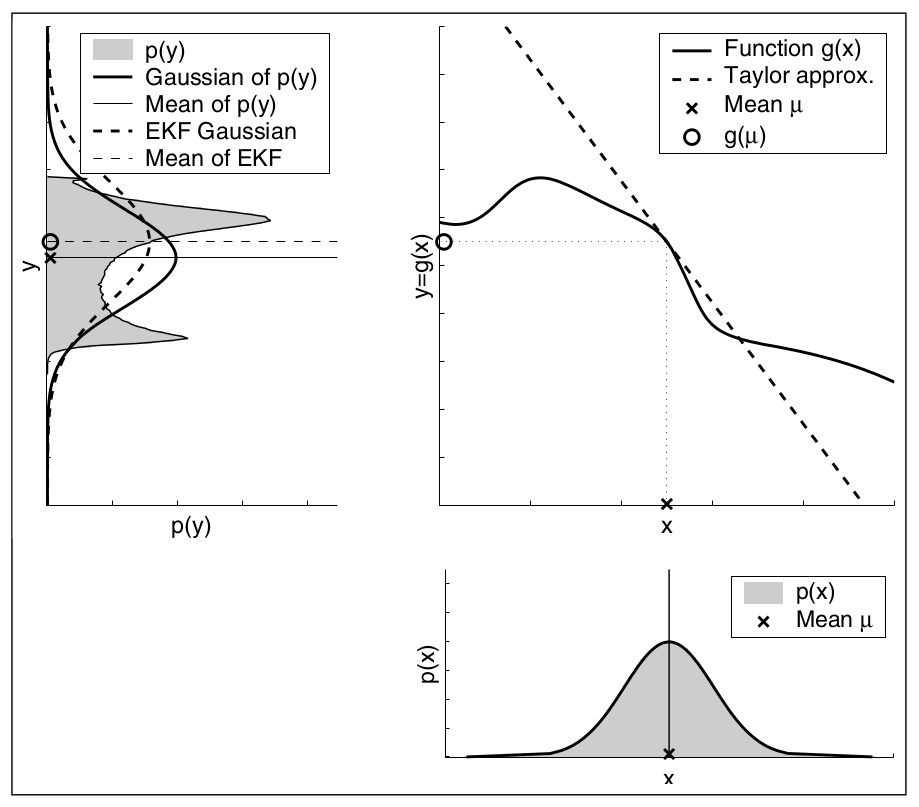
\includegraphics{Images/fig2-ekf-linearization.png}
    \caption[Linearization applied in EKF]{Linearization applied in \ac{EKF}. In this case, the nonlinear function $g$ is approximated using first order Taylor expansion, that is a linear function tangent to $g$ at the mean of the original density function. The linearization is not perfect, so it adds an error, depicted in the upper left plot. This error is the difference between the dashed line and the solid line. \cite{prob-robotics}}
    \label{fig:chapter1:kf:ekf:ekf-linearization}
\end{figure}

The Figure~\ref{fig:chapter1:kf:ekf:ekf-linearization} depicts the approximation of $g$ by a linear function that is tangent around its mean. The resulting density function is shown in the upper left plot with a dashed line, that is similar to the original density function.\\

\begin{algorithm}
    \caption{Extended Kalman Filter algorithm}
    \label{alg:chapter1:kf:ekf}

    \BlankLine
    \KwIn{$\mu_{t-1}$, $\Sigma_{t-1}$, $u_t$, $z_t$}
    \BlankLine
    $\hat\mu_t = g \left(u_t, \mu_{t-1}\right)$ \\
    $\hat\Sigma_t = G_t \Sigma_{t-1} G_t^T + R_t$ \\
    \BlankLine
    $K_t = \hat\Sigma_t H_t^T \left(H_t \hat\Sigma_t H_t^T + Q_t\right)^{-1}$ \\
    $\mu_t = \hat\mu_t + K_t \left(z_t - h \left(\hat\mu_t\right) \right) $ \\
    $\Sigma_t = (I - K_t H_t) \hat\Sigma_t$ \\
    \BlankLine
    \Return{$\mu_t$, $\Sigma_t$}
\end{algorithm}

The \ac{EKF} algorithm can be seen in Algorithm~(\ref{alg:chapter1:kf:ekf}), and it is similar to Algorithm~(\ref{alg:chapter1:kf}). The difference lies in the use of the nonlinear functions $g$ and $h$ and their Jacobians, $G_t$ and $H_t$ respectively.

\section{Simultaneous Localization and Mapping}
\label{sec:chapter1:slam}
Among all the problems faced by autonomous mobile robots, two of them are relevant for this work: localization and mapping. The former one, is related to the problem of where the robot is, while the later is related to building a map of the environment. However, in order to accurately localize itself the robot needs a map of the environment in which it is immersed in, and, in order to build a map, it needs to know where it currently is, giving us a chicken-egg situation. Hence, the \ac{SLAM} problem appears when the robot has no knowledge of its localization nor its environment map, while measurements and controls are given.\\

The problem of building a map can be summarized in the following steps:
\begin{enumerate}
    \item{The robot senses the environment using its sensors}
    \item{It creates a representation of the acquired data}
    \item{It integrates the processed sensor data with the previously learned map structure}
\end{enumerate}

While this process can be done by manually moving the robot around the environment, it is more challenging to build the map while the robot is moving autonomously. \\

%\nocite{intro-aut-mobile-robots}
On the other hand, assuming that the robot already knows the map, the localization problem could be trivial if no noise is present at all. The sensors, wheel encoders, different kinds of terrain, battery life, etc, all of these can make the robot to increase its uncertainty related to where it is. As robot moves around the environment it uses its sensors to estimate its position, increasing its uncertainty regarding its position relative to the map. At some point, the robot will "see" a known landmark or feature in the environment, correcting its position while reducing the uncertainty.\\
\begin{figure}
    \centering
    \includegraphics[width=\textwidth]{Images/fig3-slam.png}
    \caption[Example of SLAM problem]{At the beginning \textbf{(a)} the robot has low uncertainty regarding its pose. As it moves around the environment its uncertainty, represented by the dark gray ellipsis, grows \textbf{(b), (c), (d)}, until it sees a known landmark \textbf{(e)}, making the position uncertainty to shrink. \cite{intro-aut-mobile-robots}}
    \label{fig:chapter1:slam}
\end{figure}

The localization and mapping problems can be solved together by using a \ac{SLAM} technique, with which the robot will build the map while localizing itself in it. An example of this problem can be seen in Figure~\ref{fig:chapter1:slam}, where a robot moves around the environment and sees some features or landmarks. The uncertainty regarding its position is low when it starts, and keeps growing while it moves around. At the end, it sees a known landmark ($m_0$) making the uncertainty to shrink. As can be seen in the figure, the robot adds new landmarks to the map ($m_1$ and $m_2$) with their corresponding uncertainty, and when the robot sees the first landmark, not only its own uncertainty decreases, but also the two new landmarks' uncertainty. In this way, the robot's position is correlated with the observations' position estimates.\\

The idea of the \ac{SLAM} problem is to estimate a posterior belief that involves not only the robot pose, but also the map: $p\left(x_t, m | z_{1:t}, u_{1:t}\right)$, where $x_t$ is the robot's pose at time $t$, $m$ is the map, $z_{1:t}$ are the measurements, and $u_{1:t}$ are the controls given to the robot.

\subsection{EKF-SLAM}
\label{subsec:chapter1:slam:ekfslam}
The \ac{SLAM} problem can be addressed, between others, using an \ac{EKF} approach. The algorithm proceeds in the same way as shown in Section~\ref{subsec:chapter1:kf:ekf}, being $\mu$ a state vector containing the information for the robot pose ($q_r$) and the landmarks' pose ($m_i$):
\begin{equation}
    \mu = \begin{bmatrix}
        q_r & m_0 & \dots & m_{n-1}
    \end{bmatrix}^T~~.
\end{equation}

One thing that is worth mentioning is that in EKF-SLAM maps are \emph{feature based}. This means that the features or landmarks are assumed to be points in the space: if the robot sees, for example, a chair, it will store a point that represents the chair in space. Also, as explained before, it assumes Gaussian noise for the robot motion and observations.\\

The EKF-SLAM algorithm estimates the robot's pose in addition to all encountered landmarks' poses along its way. Thus, there is a correspondence between robot's pose and landmarks, and that is why it is necessary to include the landmarks information into the state vector. Hence, the algorithm estimates the posterior $p\left(\mu_t | z_t, u_t\right)$.\\

\begin{algorithm}[h]
    \caption{EKF-SLAM algorithm}
    \label{alg:chapter1:slam:ekfslam}
    \BlankLine
    \KwIn{$\mu_{t-1}$, $\Sigma_{t-1}$, $u_t$, $z_t$}
    \BlankLine
    $\hat\mu_t = g\left(\mu_{t-1}, u_t\right)$\;
    $G_t = computeJacobian\left(g\right)$\;
    $\hat\Sigma_t = G_t \Sigma_{t-1} G_t^T + R_t$\;
    \BlankLine
    \ForEach{landmark observation $z_t^i$}{
        \BlankLine
        \If{landmark $i$ has not being seen before}{
            $addLandmarkToStateVector\left( z_t^i \right)$
        }
        \BlankLine
        $H_t^i = computeJacobian\left( h^i \right)$\;
        $v^i =  z_t^i - h^i \left( \hat\mu_t \right)$\;
        $S = H_t^i \hat\Sigma_t H_t^{iT} + Q_t$\;
        $K_t^i = \hat\Sigma_t H_t^{iT} S^{-1}$ \;
        $\mu_t = \hat\mu_t + K_t^i \left( v^i \right) $ \;
        $\Sigma_t = (I - K_t^i H_t^i) \hat\Sigma_t$ \;
    }
    \BlankLine
    \Return{$\mu_t$, $\Sigma_t$}
\end{algorithm}

Assuming the robot's pose is composed by $x$, $y$, $\theta$ , the markers' pose is composed by $x$, $y$, and there are $N$ markers, the state vector $\mu$ will have a length of $3 \times 2N$, and the covariance matrix $\Sigma$ will have a size of $(3 \times 2N) \times (3 \times 2N)$.\\

The EKF-SLAM can be seen in Algorithm~(\ref{alg:chapter1:slam:ekfslam}). From lines 1 to 3, it computes the state vector and covariance matrix updates; the function $computeJacobian$ computes, indeed, the Jacobian matrix for the motion model $g$, and the resulting matrix has the same size as the covariance matrix and has the following characteristic:
\begin{align}
   G_t &= \begin{bmatrix}
        G_r & \textbf{0} \\
        \textbf{0} & \textbf{I}
    \end{bmatrix}~~,\\
    G_r &= \begin{bmatrix}
    \frac{\partial x'}{\partial \mu_{t-1,x}} & \frac{\partial x'}{\partial \mu_{t-1,y}} & \frac{\partial x'}{\partial \mu_{t-1,\theta}}\\
    \frac{\partial y'}{\partial \mu_{t-1,x}} & \frac{\partial y'}{\partial \mu_{t-1,y}} & \frac{\partial y'}{\partial \mu_{t-1,\theta}}\\
    \frac{\partial \theta'}{\partial \mu_{t-1,x}} & \frac{\partial \theta'}{\partial \mu_{t-1,y}} & \frac{\partial \theta'}{\partial \mu_{t-1,\theta}}
\end{bmatrix}~~,
\end{align}
where $\frac{\partial x'}{\partial \mu_{t-1,x}}$ is the derivative of $g$ along $x'$ dimension, taken with respect to $x$, $y$, and $\theta$ at $\mu_{t-1}$.\\

At line 4, it iterates through every observation $z_t$. At each time step $t$, a sensor obtains a set of observations $z^i$ of one of the $N$ landmarks. Each observation is associated with a map feature, and this association is accomplished by a prediction of the measurement that each feature would generate and a measure of the difference between the prediction and the sensor measurement. The prediction of the measurements can be obtained by the observation model $h^i$, which result is a vector of predicted features. If the observation $z^i$ comes from a landmark $i$, the following relation is hold:
\begin{align}
    z^i = h^i\left(x_t\right) + w^i~~,
\end{align}
where $x_t$ is the true state and $w^i$ is the observation noise with covariance $Q_t$, and assumed to be zero mean, Gaussian, additive, and independent of the process noise. If the landmark is not already in the state vector, at line 6 it is added by projecting the observation and calculating the landmark's pose, adding two new elements to the state vector and two new more columns and rows to the covariance matrix. At line 7 the Jacobian of the observation model is computed.\\

At line 8, the innovation is calculated while its covariance is calculated at line 9. The innovation measures the discrepancy between the predicted observation and the actual sensor measurement. At line 10 the Kalman gain is computed, and at line 11 the state vector is updated. The gain propagates the information through all the state vector, updating not only the robot's pose, but also the landmarks' poses.\\

The fact that the Kalman gain is not sparse is important, because observing a landmark not only improves the estimate of that landmark's pose, but also all the others, along with the robot's pose. This effect can be seen in Figure~\ref{fig:chapter1:slam}, with an additional explanation: most of the uncertainty of the landmarks' poses is caused by the robot's own uncertainty, so the location of those previously seen landmarks are correlated. When the robot gains information about its own pose, this information is propagated to the landmarks, and as result it improves the localization of other landmarks in the map.

\subsection{Adding new landmarks}
\label{subsec:chapter1:slam:ekfslam:addlandmarks}
So far, the existence and accuracy of a map was assumed. Nevertheless, this is not always true, and the construction of a map should somehow be done. EKF-SLAM algorithm includes the possibility of adding new landmarks to the map while doing the localization process with known landmarks. This process of adding new landmarks to the map is done via what is called inverse observation model, which handles the sensor measurements, identifies the new landmark, and adds it to the state vector.\\

The inverse observation model will produce the coordinates of the new landmark in the map, and this information will be added to the state vector, which will increase its size (in this case) by two new elements.
\begin{align}
    h^{-1}\left(\bm{x_r}, \bm{z}\right) &= \begin{bmatrix}
        x_l \\ y_l
    \end{bmatrix}~~,
    \label{eq:chapter1:slam:ekfslam:inverseh}\\
    \bm{x_t} = y\left(\bm{x}, \bm{z}\right) &= \begin{bmatrix}
        \bm{x} \\ h^{-1}\left(\bm{x_r}, \bm{z}\right)
    \end{bmatrix}~~.
    \label{eq:chapter1:slam:ekfslam:extension_y}
\end{align}
In equation~(\ref{eq:chapter1:slam:ekfslam:inverseh}) $\bm{x_r}$ refers to the elements in the state vector that corresponds to the robot's pose, and $\bm{z}$ refers to the observation elements, which can be, for example, range and bearing data. Since the state vector has a variable length, extending the covariance matrix is also needed whenever the robot sees a landmark that has not being seen previously. The extension of the covariance matrix is achieved as shown in equation~(\ref{eq:chapter1:slam:ekfslam:cov_update}).
\begin{align}
    \hat{\bm{\Sigma}} = \bm{Y_x} \bm{\Sigma} \bm{Y_x}^T + \bm{Y_z} \bm{Q}_t \bm{Y_z}^T~~,
    \label{eq:chapter1:slam:ekfslam:cov_update}\\
    \bm{Y_x} = \frac{\partial y}{\partial x} = \begin{bmatrix}
        \frac{\partial x}{\partial x} \\ \frac{\partial h^{-1}}{\partial x}
    \end{bmatrix} = \begin{bmatrix}
    \bm{I} \\ \bm{G_x}
    \end{bmatrix}~~,
    \label{eq:chapter1:slam:ekfslam:yx}\\
    \bm{Y_z} = \frac{\partial y}{\partial z} = \begin{bmatrix}
        \frac{\partial x}{\partial z} \\ \frac{\partial h^{-1}}{\partial z}
    \end{bmatrix} = \begin{bmatrix}
        \bm{0} \\ \bm{G_z}
    \end{bmatrix}~~,
    \label{eq:chapter1:slam:ekfslam:yz}
\end{align}
where matrices $\bm{Gx}$ and $\bm{Gz}$ are the Jacobian of function $h^{-1}$ with respect to the state vector and the observation vector respectively. By substituting the Jacobians in equations (\ref{eq:chapter1:slam:ekfslam:yx}) and (\ref{eq:chapter1:slam:ekfslam:yz}) into equation~(\ref{eq:chapter1:slam:ekfslam:cov_update}), the following matrix is obtained:
\begin{align}
    \hat{\bm{\Sigma}} = \begin{bmatrix}
        \bm{\Sigma} & \bm{\Sigma} \bm{G_x}^T \\
        \bm{G_x} \bm{\Sigma} & \bm{G_x} \bm{\Sigma} \bm{G_x}^T + \bm{G_z} \bm{Q}_t \bm{G_z}^T
    \end{bmatrix}~~.
    \label{eq:chapter1:slam:ekfslam:cov_update_full}
\end{align}\\

The linearized covariance update can be factored as shown in equation~(\ref{eq:chapter1:slam:ekfslam:factoring}) by assuming that $A \equiv 1$, $B \equiv 0$, $C \equiv 0$ and $D \equiv \bm{G_z}$
\begin{align}
    \begin{bmatrix}
        A & B \\ C & D
    \end{bmatrix} \begin{bmatrix}
        P & 0 \\ 0 & Q
    \end{bmatrix} \begin{bmatrix}
        A & B \\ C & D
    \end{bmatrix}^T &= \begin{bmatrix}
            APA^T + BQB^T & APC^T + BQD^T \\
            CPA^T + DQB^T & CPC^T + DQD^T
    \end{bmatrix}~~,
    \label{eq:chapter1:slam:ekfslam:factoring}\\
    \hat{\bm{\Sigma}} &= \begin{bmatrix}
        \bm{1} & \bm{0} \\ \bm{G_x} & \bm{G_z}
    \end{bmatrix} \begin{bmatrix}
        \bm{\Sigma} & \bm{0} \\ \bm{0} & \bm{Q}_t
    \end{bmatrix} \begin{bmatrix}
        \bm{1} & \bm{0} \\ \bm{G_x} & \bm{G_z}
    \end{bmatrix}^T~~.
    \label{eq:chapter1:slam:ekfslam:factored_cov_update}
\end{align}

\section{Normalized Estimation Error Squared}
\label{sec:chapter2:nees}
The Mahalanobis distance is a measure of the distance between a point and a distribution. It is a way to measure how many standard deviations is away the point from the mean of the distribution. The Mahalanobis distance of an observation $\bm{x} = \begin{bmatrix}x_1 & x_2 & \dots \end{bmatrix}$ with mean $\bm{\mu} = \begin{bmatrix}\mu_1 & \mu_2 & \dots \end{bmatrix}$, and covariance matrix $\Sigma$ is defined as:
\begin{equation}
    D = \sqrt{\left(\bm{x} - \bm{\mu}\right) \Sigma^{-1} \left(\bm{x} - \bm{\mu}\right)}~~.
    \label{eq:chapter1:nees:mahalanobis}
\end{equation}

Every time the drone observes a landmark, a node responsible of identifying it processes the features that distinguish it with respect to other landmarks, and publishes these features as a message. In the case of poles, range and bearing information is provided, while in the case of markers the position and orientation information with respect to the camera frame is provided. Given this, each observation $z$ for a pole, is composed by three measurements, and each observation of a marker is composed by six measurements. After observing a landmark the Algorithm~(\ref{alg:chapter1:slam:ekfslam}) calculates the discrepancy between the observation $i$ and the predicted observation by the innovation ($v^i$), and its covariance ($S$), as
\begin{align*}
    v^i =  z_t^i - h^i \left( \hat\mu_t \right)~~,\\
    S = H_t^i \hat\Sigma_t H_t^{iT} + Q_t~~.
\end{align*}

The square of the Mahalanobis distance can be used in order to establish a correspondence between the observed measurements with the landmark features if the following holds:
\begin{align}
    D_i^2 = v^i S^{-1} v^i < \chi_{d, 1-\alpha}^2~~,
    \label{eq:chapter2:nees:innov_test}
\end{align}
where $d$ is the size of $h^i$ and $1-\alpha$ is the desired confidence level. This test is called individual compatibility, and when applied to the predicted state can be used to determine the subset of observation features that are compatible with the observation.\\

Furthermore, a state estimate is consistent if its state estimation error $\bm{x} - \hat{\bm{x}}$ satisfies
\begin{align*}
    \mathbb{E}\left[\bm{x} - \hat{\bm{x}}\right] = 0~~,\\
    \mathbb{E}\left[\left(\bm{x} - \hat{\bm{x}}\right)\left(\bm{x} - \hat{\bm{x}}\right)^T\right] \le \Sigma~~.
\end{align*}
When the ground truth $\bm{x}$ is available, a \ac{NEES} can be performed to check the consistency of the filter. \ac{NEES} test can be defined as the squared Mahalanobis distance for the difference between $\bm{x}$ and $\hat{\bm{x}}$, and consistency can be checked with a $\chi^2$ test
\begin{align*}
    NEES = \left(\bm{x} - \hat{\bm{x}}\right) \Sigma^{-1} \left(\bm{x} - \hat{\bm{x}}\right) \le \chi_{d, 1-\alpha}^2~~.
\end{align*}

However, the ground truth is only available in simulated environments thus, the consistency of the filter is maintained by using observations that satisfy the test in equation~(\ref{eq:chapter2:nees:innov_test}). This way, the filter will discard observations that do not satisfy the innovation test, maintaining a consistent estimation of the state and therefore, the map.
